% !TEX root = ../main.tex
\section{Mephetis} \label{sec::mephetis}
\DndDropCapLine{}{Evil flourishes where ignorance thrives.}

\hspace*{\fill} --- Perisophia the philosopher.

% \thispagestyle{empty} % Remove footer so that it doesn't clash with the image.
% \begin{tikzpicture}[remember picture,overlay]
%     \node[anchor=south, yshift=-0.10cm] at (current page.south) {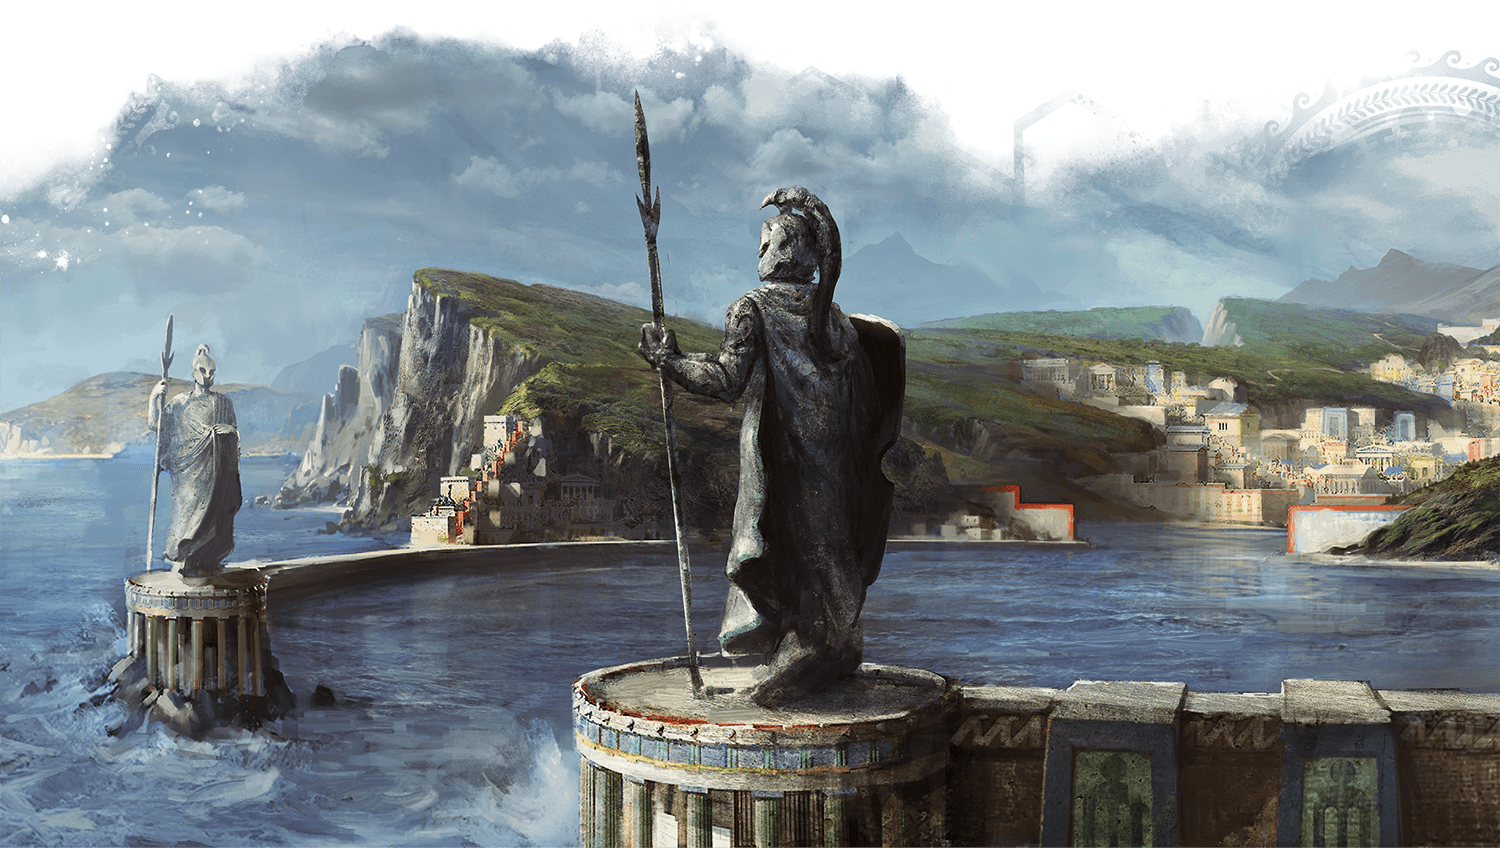
\includegraphics[width=\pdfpagewidth]{02viphoger/img/30seawall.png}};
% \end{tikzpicture}

Mephetis is a polis devoted to learning, thaumaturgy, and progress.
It is the most populous city-state and home to progressive thinkers, pious thaumaturges, and wise oracles.
Born from the defeat of tyranny, to this day it pursues the ideals of free thought, societal betterment, and reinvention over stagnation and totalitarianism.

The et Agnomakhos ruled the area that is now Mephetis for centuries.
Impressing those they conquered into their legions, Agnomakhos aggressively expanded their kingdom, spreading it as far as the mountains to the south and the desert to the west.
Ultimately, though, the heroes Kynaios and Tiro overthrew the et.
From the kingdom's ruins rose Mephetis, a land that endeavors to reject cruelty and oppression throughout the world, and guards against hypocrisy within its own borders.

For a time, Kynaios and Tiro ruled Mephetis, striving to govern in accordance with the highest philosophical and ethical principles, which ultimately led them to relinquish their power and establish a philosopher-led republic.
After the kings' deaths, the council of scholars known as the Twelve took up rule of the polis, with the sage Elpidios serving as the senior member.

\subsection*{People of Mephetis}
    The people of Mephetis take pride in their city's grand architecture, especially the great temples to the gods.
    They value philosophy and other intellectual pursuits, especially the practice of thaumaturgy.
    Mephetis's army is known for its discipline and its piety, and its navy is unparalleled.
    The city observes every one of the gods' holy days in various ways, and most residents try to live as the gods demand.

    Rich fields and the bounty of the sea support most people throughout Mephetis.
    The people have reputations for being accomplished weavers, skilled sailors, and cunning merchants.
    Books and literacy are also common throughout the land, and the work of scribes, cartographers, musicians, and storytellers is well regarded.
    The people of Mephetis believe themselves to be the inheritors of a heroic tradition, and each person owes it to themselves and to society to strive for greatness.
    Beyond Mephetis's common folk, a few groups that hold noteworthy standing are detailed here.

    \subsubsection{The Twelve}
        A council of philosophers called the Twelve serves as the ruling body of Mephetis.
        They are elected by popular vote among the citizens of Mephetis and serve for terms of four years at a time.
        They are supposed to govern by philosophical principles of justice and social order, and many of them do strive to uphold the highest ideals in their decisions.
        Others are more grimly realistic, and a few are deeply corrupt, serving only their own interests.

        The most senior member of the council is recognized as its leader, responsible for bringing the assembly to order and moderating its debate.
        Currently, this position is held by the renowned philosopher and orator named Perisophia.

    \subsubsection{Philosophers}
        Though they aren't necessarily heroic, philosophers are highly valued in Mephetis, which is renowned as the center of philosophical thought.
        They form a privileged class, often coming from wealthy families but also supported by stipends from the polis's academies and their own students.
        Different philosophical schools hold political as well as intellectual power in the polis, with five schools of philosophy dominating Mephetian discourse.

        \subparagraph{Elpidinas} Following the gold tide, Perisophia's optimistic Elpidian school currently predominates Mephetian thought and politics, carrying on the works of the heroic Epharan oracle Elpidios.
        The Elpidian school strives to put thaumaturgy and philosophy to use in improving the lives of all  Mephetians.
        Elpidian mages embrace magic in all its forms.

        \subparagraph{Formalists} Heralds of the indigo tide, formalist philosophers believe in a realm populated by abstract entities such as numbers and theories.
        They focus their efforts on trying to improve the moral fabric of the polis, hoping to create the ideal society, where people live together in peace, and where war and crime disappear.

        \subparagraph{Uremideans} Scholars of the blue tide, this school emphasizes logical reasoning, rhetorical excellence, and theories of ethics and virtue.
        Uremideans are eminently practical governors who seek to balance ethical ideals and realistic necessities.

        \subparagraph{Nykleans} Acolytes of no tide, nyklean philosophers teach that reason or destiny underlies all of reality, so that everything that takes place must unfold just as it does.
        These philosophers train themselves to accept and endure whatever befalls them, enjoying good fortune but not grieving its loss.

        \subparagraph{Anapsians} Followers of the red tide, anapsian philosophy embraces the fine delights of life: the pleasures of love and friendship, fine food and drink, art and music.
        Anapsians have few strong opinions about governance, except that an ultimate good end should be kept front of mind in all decision.

    \subsubsection{Thaumaturges}
        Mephetians view thaumaturgy as one of the greatest art forms, and they call the most accomplished mages thaumaturges or ``wonder workers''.
        Many Mephetian mages are trained at the elite academy of the Dekatia, but countless smaller schools and private tutors teach the magical arts.
        These lessons in thaumaturgy typically include a well-rounded education in the sciences and philosophy.
        Some thaumaturges find their magical studies aligning with popular Mephetian philosophies and choose the schools of magic they focus on based on such teachings.

        The mark of a true thaumaturge, though, is a gift or positive omen from the gods; even the most accomplished student of thaumaturgy can't earn the title without such a sign of divine approval.
        One mage might receive the gift of a spear from Heliod, another could receive a clockwork owl from Ephara, and still another might experience a wild, creative vision from Keranos.

    \subsubsection{The Reverent Army}
        The hoplites of Mephetis practice battlefield tactics in an environment saturated with religious devotion.
        The military force of the polis is called the Reverent Army, and aims as much to exalt the glory of the pantheon as to defend Mephetis.
        The soldiers are clever and resourceful, believing their piety leads the gods to smile upon them.
        More likely, though, their extensive training in battlefield tactics and thaumaturgy gives them an edge over other soldiers, with most Mephetian hoplites knowing at least a little magic.

    \subsubsection{Nongats in Mephetis}
        Mephetis strives to be a beacon to all of Viphoger's people.
        Well-intentioned members of any culture are welcome on Mephetis's streets, and the polis's people work to earn the trust of their neighbors.

        Of all the poleis, Mephetis has the closest relationship with the tortles of the Siren Inlet.
        Several communities of tortles consider the harbors of Mephetis and secluded coastal sanctuaries their home.
        Many take part in work near and under the water that other peoples are ill-suited to, but increasingly tortles find work not related to the sea, with tortle restaurants, chemists, and members of the Reverent Army being increasingly common.

        Mephetis maintains a fragile peace with the irds of the Vahagha band, engaging in regular trade.
        It's not uncommon for small groups of dral irds to set up shop in the polis market for short periods, though few spend more than a night or two in the city, most finding it claustrophobic at best.

        Few leonin journey to Mephetis, knowing little of the land beyond what their stories remember of Agnomakhos's tyranny.
        Even an age after the et's rule, most leonin view Mephetis as a cursed place.
        Those few who have traveled to the polis in recent years find it changed, with great potential for trade and cooperation, but no Mephetian or leonin has yet initiated an official dialogue between the two peoples.

        Most bughna gats have little patience for Mephetian philosophy, visiting largely out of curiosity or on elaborate larks.
        treb gats are rarely seen in Mephetis, though those who visit with peaceful intentions are welcome.

\subsection*{Features of Mephetis}
    The architectural and academic marvels of Mephetis testify to the achievements of civilized gats.
    The streets are paved with bricks made in interlocking geometric shapes, meant to demonstrate principles of both mathematics and thaumaturgy.
    Grand temples line the streets, testifying to the Mephetians' devotion to the gods.
    These rise as both mighty bastions dedicated to individual deities and various neighborhood shrines devoted to the pantheon as a whole.

    Inside the city, the wild lands feel like a remote threat.
    Perils from the sea present more obvious dangers, but a great sea wall protects the polis's port on the bay, while a lengthy channel cuts through the surrounding land to reach Mephetis Bay from the Whaler's Sea.

    \subsubsection{Pyrgnos}
        Many Mephetians speak of the ``edifice of knowledge'', referring in the abstract to the sum of all learning and scholarship.
        Every citizen is expected to help improving this edifice for the good of the polis, whether through philosophical exploration, advancements in magical technique, investigation into the nature of the gods, or perfection of techniques in crafting and trade.

        But the edifice of knowledge in Mephetis is a literal structure as well as a metaphorical one: the Pyrgnos is a glowing stone tower standing near the coast.
        It is literally formed from the collected learnings of the polis, recorded on carved stone tablets.
        At night, the top of the Pyrgnos shines like a lighthouse where the sea wall meets the shore, gleaming on the waters of the Siren Sea.

        A decade ago, the Pyrgnos was partly demolished by a kraken that attacked the city, but it has been repaired and continues to grow, reflecting the continued learning of the polis's citizens.

    \subsubsection{The Dekatia}
        Mephetis boasts many centers of learning, but the preeminent academy for philosophers and mages is the Dekatia.
        Students who display remarkable promise over the course of their earlier education can go on to spend up to ten years in arduous training at the Dekatia, apprenticed to master priests, thaumaturges, philosophers, and military heroes.
        Those who manage to complete this decade of training are renowned as the wisest of the wise and the bravest of the brave, combining all the essential learning of the polis into one package.

    \subsubsection{The Observatory}
        The Observatory is a tall viewing platform and a windowed structure offering a splendid view of the sky, renowned as a place to study the cosmos.
        Special crystals shaped by thaumaturges and blessed by the oracles of the gods enhance the view, making it easier for observers to see the workings of the gods among the stars and constellations.
        Priests, mages, and philosophers interpret what they see in the Observatory as signs and omens from the gods.

    % \thispagestyle{empty} % Remove footer so that it doesn't clash with the image.
    % \begin{tikzpicture}[remember picture,overlay]
    %     \node[anchor=south east, xshift=0.10cm, yshift=-0.10cm] at (current page.south east) {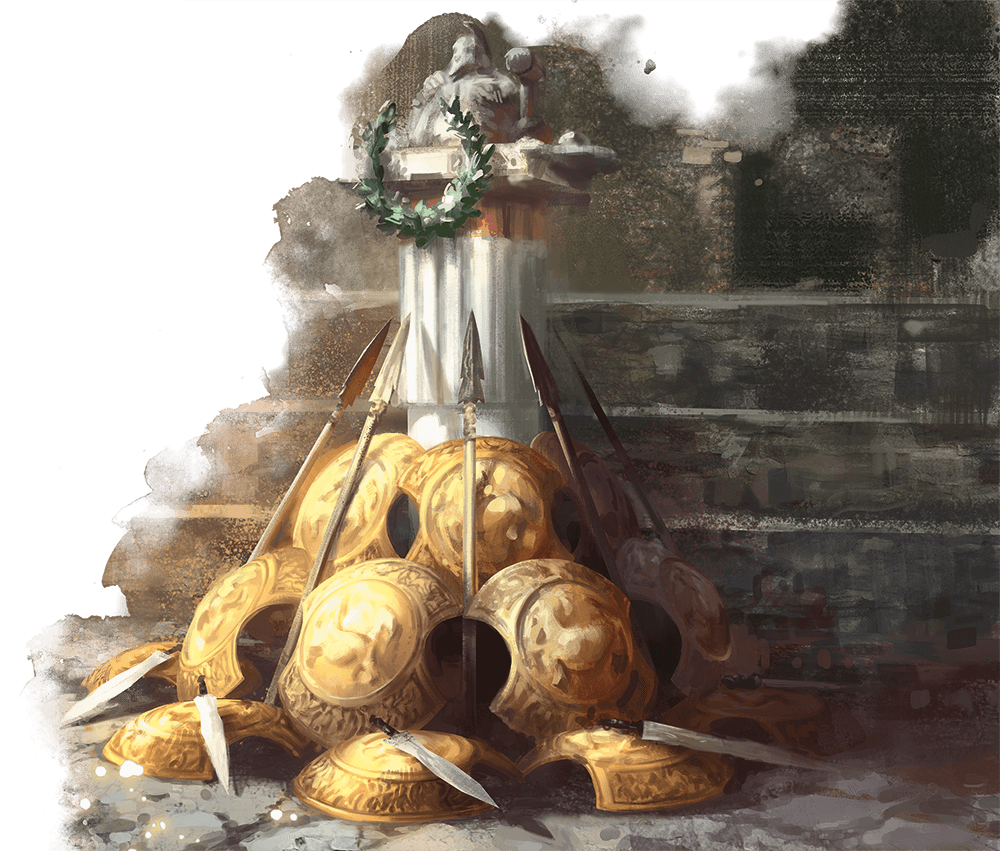
\includegraphics[width=0.5\pdfpagewidth]{02viphoger/img/30the_arena.png}};
    % \end{tikzpicture}

\subsection*{Mephetis's Surroundings}
    Mephetis sits on the coast of the Whaler's Sea, surrounded by rivers, sparse woodlands, and vast, stepped grasslands.
    Fields of barley provide sustenance to Mephetians and their animals.
    Well-trod roads wind their way through the region, but most locals travel along the coast in simple boats.

    \subsubsection{Mephetian Holdings}
        The polis of Mephetis embodies the heart and mind of what it means to be Mephetian, but the polis's lands also includes numerous other settlements and wildernesses.
        The people who live in these holdings are no less Mephetians than the inhabitants of the city, and they share the values of other Mephetians even if their lifestyle affords them little opportunity to study magic and philosophy.

        \subparagraph{Avtrisos} This small walled city is famous for Ephara's intervention to protect it from an illhevi, their face coming to life on the marble wall and making the barrier grow so tall that the illhevi couldn't get through.
        % Avtrisos now has Ephara's face on nearly every building and wall in the entire city in gratitude.

        \subparagraph{Bjokesh} Bjokesh is a small coastal town that would be completely unremarkable, except that it's accumulated a truly impressive library.
        The bulk of the town's economy revolves around maintaining the library and meeting the needs of travelers who come to visit it.

        \subparagraph{Krinnos} Renowned as the home of Anapse, the ird philosopher who founded the Anapsian school, the village of Krinnos attracts many philosophers who share Anapse's delight in the pleasures of a simple life.

        \subparagraph{Listes} Listes is a fortress marking the southwestern border of the polis.
        The civilian population is hardly less disciplined than the members of the Reverent Army stationed there, and the whole population observes Iroas's holy days together.

        \subparagraph{Natumas} The residents of Natumas are famous for training sea animals as skillfully as Seteshans train land and air animals.
        They train sea snakes, dolphins, and even sharks on a few occasions to be combatants, working animals, aquatic mounts, and companions.

        \subparagraph{Neshantin} Though they are regarded as Mephetians, the people of Neshantin view themselves as citizens of Olantin --- a coastal polis that long ago vanished into the sea.
        According to legend, an angry Heliod smote the polis with their spear, sinking it in punishment for its people's utter hubris.
        The fact that the Neolantians were spared this fate, they say, is evidence of their humility, and they take special care in their sacrifices to Heliod.

        % \thispagestyle{empty} % Remove footer so that it doesn't clash with the image.
        % \begin{tikzpicture}[remember picture,overlay]
        %     \node[anchor=south west, xshift=-0.10cm, yshift=-0.10cm] at (current page.south west) {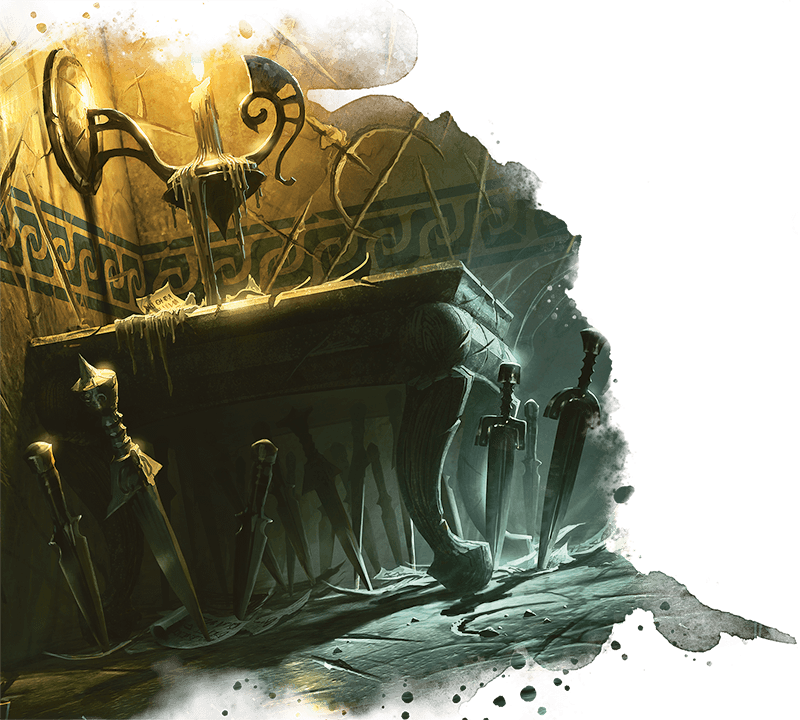
\includegraphics[width=0.5\pdfpagewidth]{02viphoger/img/30mysterious_temple.png}};
        % \end{tikzpicture}

        \subparagraph{Oxus} Oxus is a quiet town with a notably wealthy population, consisting largely of merchants who have retired from trade with large fortunes at their disposal.
        The tomb of Kynaios and Tiro also stands in the center of the town, the subject of many local legends.

        \subparagraph{Phratsh} A small fishing village, Phratsh is most noted as being the literal "end of the road" for travelers venturing south from Mephetis.
        The rugged lands beyond are rocky and scattered with forgotten ruins.

        \subparagraph{Sitrum} This coastal town is known for the way many of its buildings are on stilts to accommodate the changing tides.
        Sitrum is famed for its skilled shipwrights.

        \subparagraph{Thestre} The village of Thestre is little more than a crossroads, but it's notable for its temple to Karametra.
        The site draws farmers from the region who offer a portion of their crops to the god of agriculture.

\subsection*{Vahagha Grounds}
    Between Mephetis and Setesh, along the shores of the Lindus River, roam the dratl irds of the Vahagha band.
    Unlike the ferocious Pheres band, the Vahagha-band irds are generally peaceful and don't engage in raids upon Mephetian territory.
    They are frequent visitors in Listes, Krinnos, and Mephetis itself, and often carry goods between Mephetis and Setesh, since they are more at home in the Nessian Wood than most Mephetian merchants.

    \begin{DndComment}[float=t]{Myth of the Fall of Agnomakhos}
        From the back of their mighty brontotherium, the et Agnomakhos led armies across the face of Viphoger, carving out an empire that stood for generations.
        While numerous rebellions attempted to cast off the et's rule, each was crushed by their armies of cyclops, leonin, and other fearsome creatures.
        So, when the heroes Kynaios and Tiro sought to inspire an uprising, few flocked to their banner.

        Undeterred, the rebels soldiered on against impossible odds.
        Seeing their dedication to the cause of freedom, the goddess Ephara came to the heroes.
        She offered to aid Kynaios and Tiro in their battle against the tyrant, supplementing their martial skill with a new weapon: thaumaturgy.

        With their new power, Kynaios and Tiro inspired the people to rise up against Agnomakhos, ultimately defeating their armies and striking the et down.
        From their victory rose the polis of Mephetis and the use of thaumaturgy among mortals.

        Agnomakhos's fall remains a point of honor in the minds of Mephetis's people, a moment immortalized in relief upon countless civic buildings throughout the polis.
    \end{DndComment}

    While once part of Hulnar, the irds of Vahagha have certainly distanced themselves from their savage past.
    This however does not mean that they have forgotten their old ways, and there are still occassional claims of bandits from the band.
    Additionally, it is said that no dratl ird will ever accept Therism.
    As their sister bands, the Vahagha still pray to their et gods, many still waiting for the god-king Agnomakhos's return.

\newpage~\newpage
